\hypertarget{sensInit_8cpp}{}\section{src/sens\+Init.cpp File Reference}
\label{sensInit_8cpp}\index{src/sens\+Init.\+cpp@{src/sens\+Init.\+cpp}}


Thread initializing sensors read at the given frequency.  


{\ttfamily \#include \char`\"{}sens\+Init.\+hpp\char`\"{}}\newline
{\ttfamily \#include \char`\"{}Event\+Queue.\+h\char`\"{}}\newline
{\ttfamily \#include \char`\"{}Event.\+h\char`\"{}}\newline
Include dependency graph for sens\+Init.\+cpp\+:\nopagebreak
\begin{figure}[H]
\begin{center}
\leavevmode
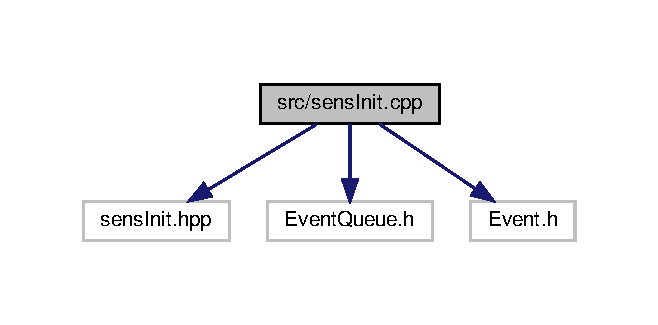
\includegraphics[width=316pt]{sensInit_8cpp__incl}
\end{center}
\end{figure}


\subsection{Detailed Description}
Thread initializing sensors read at the given frequency. 

Creates a timer that calls an interrupt with the given frequency 